
% \section{Project Schedule}

% \begin{minipage}{\linewidth}
%   \centering
%   \begin{sideways}
%     \scalebox{0.8}{

% \begin{ganttchart}[
% hgrid,
% % vgrid,
% x unit=2mm,
% % y unit title=0.3mm,
% y unit chart=7mm,
% time slot format=isodate,
% ]{2021-12-18}{2022-3-31}
% \gantttitlecalendar{year, month=name, } \\


% \ganttbar{}{2021-12-18}{2022-3-12}
% \ganttgroup[inline=false]{Draft Proposal}{2021-12-18}{2022-01-07}\\ 
% \ganttbar[progress=100,inline=false]{Literature Review}{2021-12-18}{2022-01-05}\\
% \ganttmilestone[inline=false]{Proposal Submission}{2022-01-05} \\
% \ganttbar[progress=100,inline=false]{Prepare Slides}{2021-12-18}{2022-01-07}\\
% \ganttmilestone[inline=false]{Proposal Defense}{2022-01-07} \\



% \ganttbar{}{2021-12-18}{2022-02-20}
% \ganttgroup[inline=false]{Implementation}{2022-01-07}{2022-02-20}\\ 
% \ganttbar[progress =100, inline=false]{Dataset Analysis}{2022-01-12}{2022-01-15}\\
% \ganttbar[progress =100, inline=false]{OpenPoseSkip-100}{2022-01-15}{2022-01-20}\\
% \ganttbar[progress =100, inline=false]{AnnotationInterface}{2022-01-20}{2022-01-30}\\
% \ganttbar[progress =100, inline=false]{FullBodyTagging}{2022-01-30}{2022-02-05}\\
% \ganttbar[progress =100, inline=false]{VideoPose3D}{2022-02-05}{2022-02-10}\\
% \ganttbar[progress =100, inline=false]{NeckAnnotation}{2022-02-10}{2022-02-16}\\
% \ganttbar[progress =100, inline=false]{OpenPoseFullFrame}{2022-02-16}{2022-02-19}\\

% % \ganttbar[progress =100, inline=false]{Feature Profiling}{2022-02-16}{2022-02-25}\\
% % \ganttbar[progress =0, inline=false]{Model Design}{2022-02-20}{2022-02-30}\\
% \ganttbar[progress =100, inline=false]{ Mid-Term Report}{2022-02-20}{2022-02-22}\\

% \ganttmilestone[inline=false]{Mid-term Defense}{2022-02-25} \\


% \ganttbar{}{2022-02-26}{2022-3-12}
% \ganttgroup[inline=false]{Modeling}{2022-02-26}{2022-03-12}\\ 
% \ganttbar[ progress =100, inline=false]{Training/Evaluation}{2022-02-26}{2022-03-12}\\


% \ganttbar{}{2022-3-12}{2022-3-18}
% \ganttgroup[inline=false]{Documentation}{2022-03-12}{2022-03-18}\\ 
% \ganttbar[progress =100,
% inline=false]{Report Preparation}{2022-03-12}{2022-03-18}\\

% \ganttmilestone[inline=false]{Final Defense}{2022-03-30} \\



% % \ganttgroup[inline=false]{2022-01-01}{2021-01-10} \\                  
% % \ganttbar[progress=2,inline=false]{test1}{2022-01-01}{2021-01-10}  \\  
% % \ganttmilestone[inline=false]{Milestone 2}{2022-01-01} \\             
% % \ganttbar[progress=5,inline=false]{test2}{2022-01-01}{2021-01-10}  \\ 
% % \ganttmilestone[inline=false]{Milestone 3}{2022-01-01} \\             


% % \ganttgroup[inline=false]{Group 3}{2022-01-10}{2021-02-10}  \\ 
% % \ganttbar[progress=90,inline=false]{Task A}{2022-01-10}{2021-02-10} \\ 
% % \ganttbar[progress=50,inline=false, bar progress label node/.append style={below left= 10pt and 7pt}]{Task B}{2022-01-10}{2021-02-10} \\ \\
% % \ganttbar[progress=30,inline=false]{Task C}{2022-01-10}{2021-02-10}\\ 
% % \ganttbar[progress=70,inline=false]{Task D}{2022-01-10}{2021-02-10} \\ 


% \end{ganttchart}
% }
% \end{sideways}
% \captionof{figure}[Gantt Chart showing Expected Project Timeline.]{
% Gantt Chart showing Expected Project Timeline.
% }
% \end{minipage}
%  \newpage

 \section{ Project Schedule}

 We commenced our project with detailed topic discussions, followed by an in-depth feasibility study and a comprehensive project scope evaluation. Despite encountering some minor delays during the completion phase, we have managed to align with our projected timeline and are progressing as planned. Looking ahead, we are determined to maintain this positive trajectory and successfully accomplish our forthcoming tasks


\begin{figure}[H]
\centering
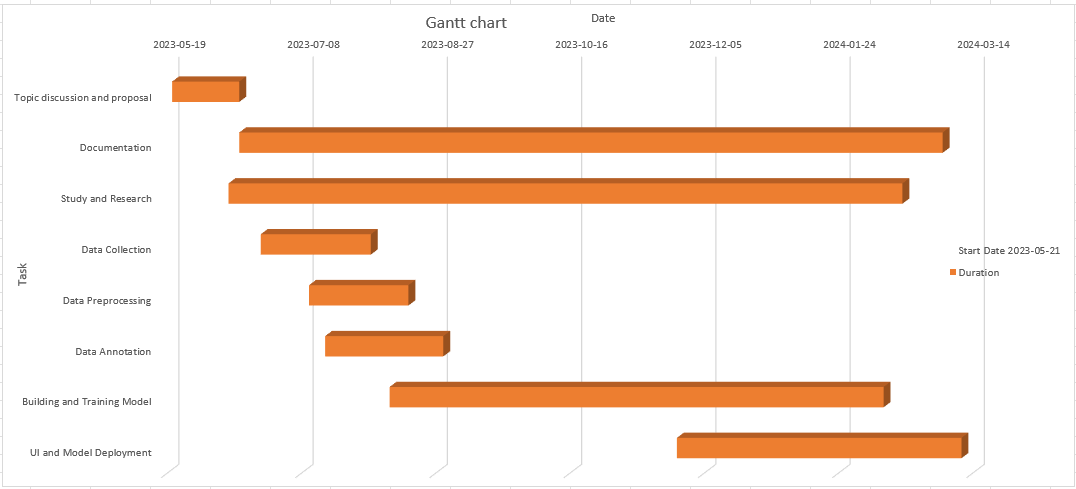
\includegraphics [scale=0.75]{img/appendix/Gantt Chart of work scheduling.png}
 \caption[Gantt Chart of work scheduling]{Gantt Chart of work scheduling}
% \label{fig:DisplaCy.png}

\end{figure}

 

\begin{table}[H]
  
\caption{ Working Progress with Percentages}
\label{tab:  Working Progress with Percentages}
    \centering
    
    \begin{tabular}{|c|c|c|}
        % \hline
        % Column 1 & Column 2 & Column 3 \\
        % \hline
        % Row 1, Cell 1 & Row 1, Cell 2 & Row 1, Cell 3 \\
        % Row 2, Cell 1 & Row 2, Cell 2 & Row 2, Cell 3 \\
        % \hline
    \end{tabular}
    
    
\end{table}


\begin{figure}[H]
\centering
\includegraphics [scale=0.59]{img/appendix/Working Progress with Percentages.png}
 %\caption[Working Progress with Percentages]{Working Progress with Percentages}
% \label{fig:DisplaCy.png}

\end{figure}
 
   

 
